\documentclass{weekly}
\begin{document}
\maketitlew{Аналитическая механика}{1}{4}{14}

\begin{wrapfigure}[6]{r}{4.7cm}\vspace{-4mm}
    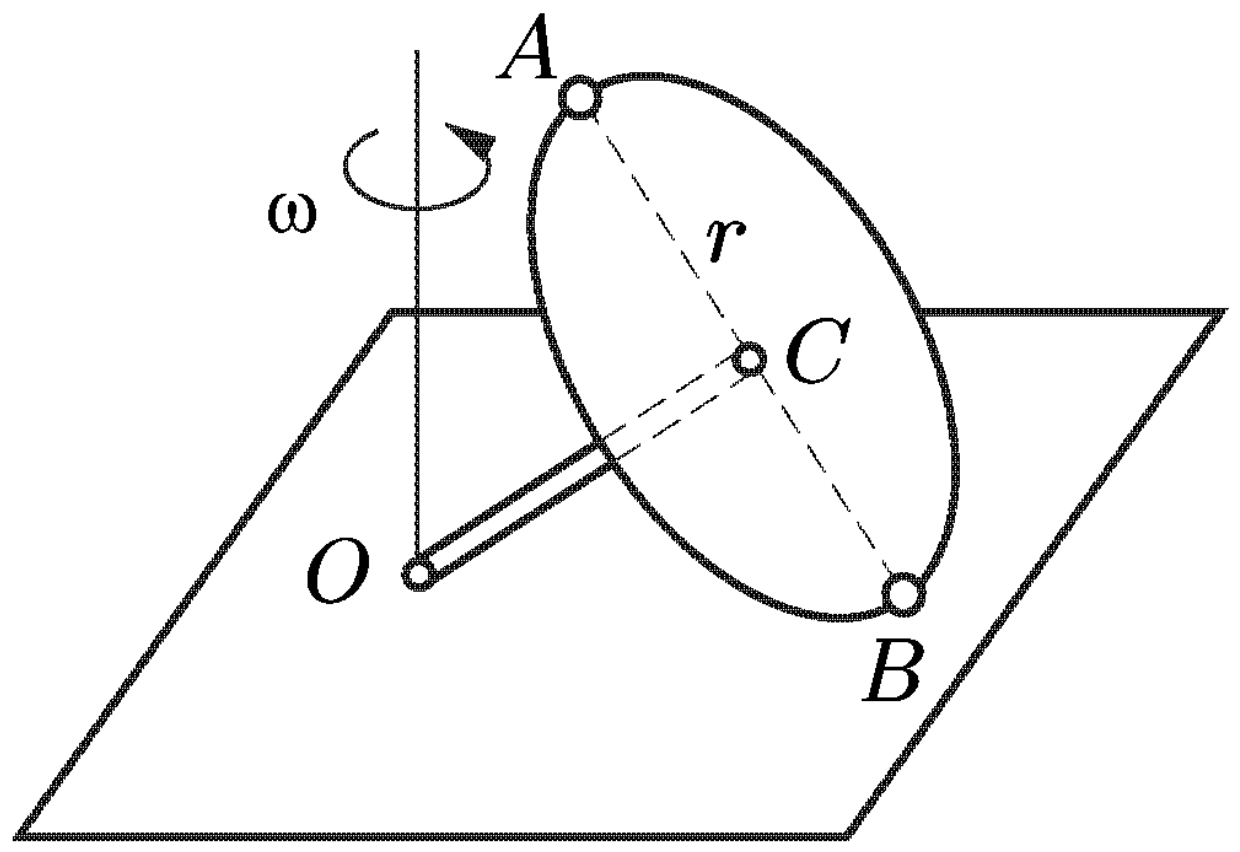
\includegraphics[width=\lw]{4-10}
\end{wrapfigure}
\paragraph{4.10.} Коническое колесо радиуса~$r$, жёстко насаженное
на~стержень~$OC$ длины $l = r\sqrt{3}$, катится по~горизонтальной
плоскости без~скольжения. Стержень~$OC$ описывает коническую поверхность,
вращаясь вокруг неподвижной точки~$O$ (в~точке~$O$ сферический шарнир)
с~угловым ускорением~$\varepsilon$, имея в~данный момент
угловую скорость~$\omega$. Определить угловые скорость и~ускорение
колеса и~ускорения его точек~$A$ и~$B$.

$\blacktriangleright$
Стержень~--- твёрдое тело с~неподвижной точкой~$O$, вращающееся
с~угловой скоростью~$\vec\omega$. С~другой стороны, колесо катится
без~проскальзывания, так~что~$\vec v_B = \overline{0}$.
В~таком случае,
\begin{align}
    \vec v_C &= \vec\omega \times \overline{OC}
        = \vec\Omega \times \overline{BC}; \label{4.10:vC}\\
    \vec w_C &= \vec\varepsilon \times \overline{OC} +
            \vec\omega \times \vec\omega \times \overline{OC}.
\end{align}
где~$\vec\Omega$~--- искомая угловая скорость колеса.
Из~уравнения~\eqref{4.10:vC} найдём её компоненты,
введя правую декартову систему координат~$Oxyz$
(ось~$Ox \upuparrows OB$, ось~$Oz \upuparrows \vec\omega$):
\begin{align}
    \cvec{0}{0}{\omega} \times \cvec{3/2}{0}{\sqrt{3}/2} r &=
            \cvec{\Omega_x}{\Omega_y}{\Omega_z} \times
            \cvec{-1/2}{0}{\sqrt{3}/2} r; \\
    \cvec{0}{3\omega}{0} &=
            \cvec{\sqrt{3}\Omega_y}{\Omega_z-\sqrt{3}\Omega_x}{\Omega_y}.
\end{align}
Видим, что~$\Omega_y = 0$.
Заметим также, что~$\vec v_C = \vec\Omega \times \overline{OC}$,
поскольку колесо движется в~целом как~твёрдое тело:
\begin{align}
    \cvec{0}{\Omega_z - \sqrt{3}\Omega_x}{0} =
            \cvec{\Omega_x}{0}{\Omega_z} \times
            \cvec{3}{0}{\sqrt{3}}
        = \cvec{0}{3\Omega_z - \sqrt{3}\Omega_x}{0}.
\end{align}
Теперь с~необходимостью $\Omega_z = 0$, так~что
$\vec\Omega = -\sqrt{3}\omega \hat x$.

\textsl{Примечание.} Как~направление, так~и~модуль угловой скорости
колеса можно было указать, в~принципе не~совершив никаких вычислений.
С~другой стороны, приведено относительно строгое доказательство
утверждения из~абзаца~1 решения задачи~4.34 (может быть применено
по~аналогии).

Найдём теперь угловое ускорение колеса:
\begin{align}
    \vec{\mathscr{E}} &= \dot{\vec\Omega}
        = -\sqrt{3} \dot\omega \hat x -
            \sqrt{3} \omega \left(\vec\omega \times \hat x\right)
        = -\sqrt{3} \left( \varepsilon \hat x + \omega^2 \hat y \right);
\\
    \mathscr{E} &= \sqrt{3 \left(\varepsilon^2 + \omega^4\right)}.
\end{align}

Ускорения точек~$A$ и~$B$ колеса могут быть рассчитаны
по~формуле Ривальса:
\begin{align}
    \vec w_A &= \vec{\mathscr{E}} \times \overline{OA} +
            \vec\Omega \times \vec\Omega \times \overline{OA}
        = \subst{\overline{OA} = r\hat x + \sqrt{3}r \hat y}
        = \cdots; \label{4.10:wA} \\
    \vec w_B &= \vec{\mathscr{E}} \times \overline{OB} +
            \cancel{\vec\Omega \times \vec\Omega \times \overline{OB}}
        = -\sqrt{3} \left( \varepsilon \hat x + \omega^2 \hat y \right)
            \times 2r \hat x
        = -2\sqrt{3} \omega^2 r. \label{4.10:wB}
\end{align}

\textbf{Ответ:}\quad $\vec{\Omega} = -\sqrt{3}\omega \hat x$;\qquad
$\vec{\mathscr{E}} = -\sqrt{3} \left( \varepsilon \hat x +
\omega^2 \hat y \right)$;\qquad \eqref{4.10:wA} -- \eqref{4.10:wB}.
\hfill $\blacktriangleleft$


\begin{wrapfigure}[13]{l}{6cm}\vspace{-2mm}
    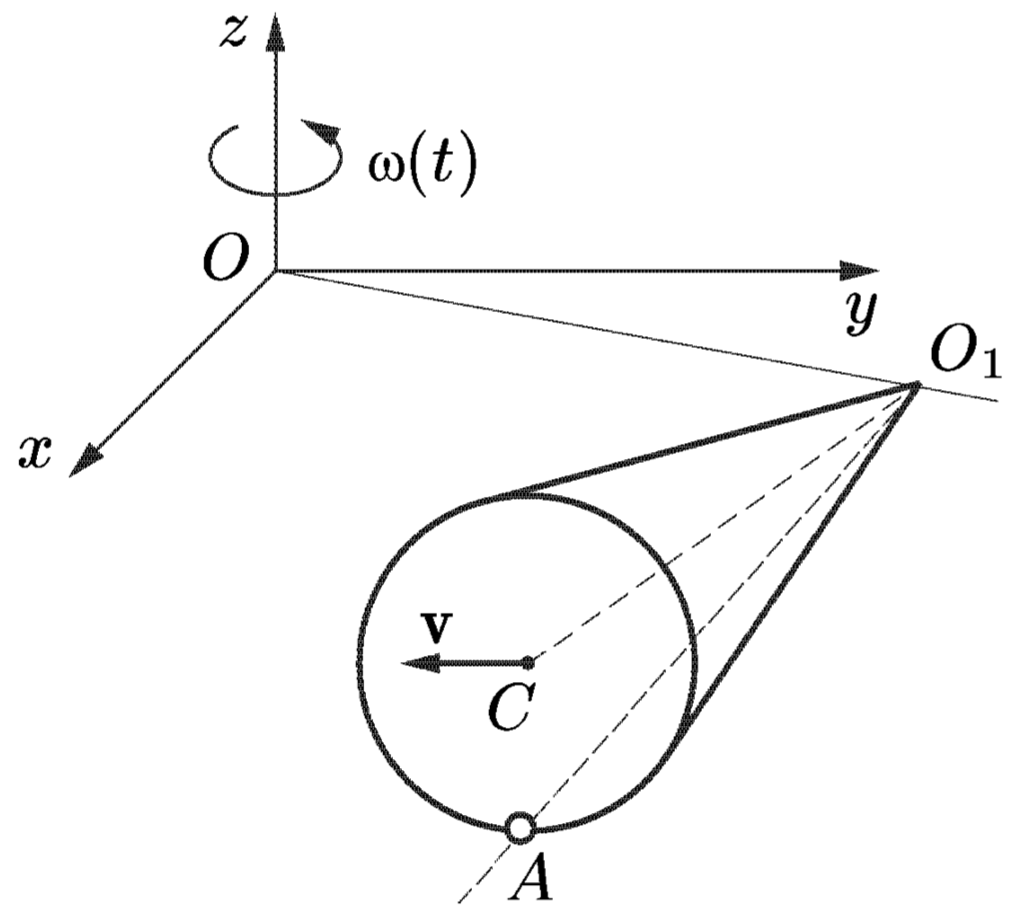
\includegraphics[width=\lw]{4-25}
\end{wrapfigure}
\paragraph{4.25.} Горизонтальная плоскость вращается вокруг
вертикальной оси~$Oz$ с~угловой скоростью~$\omega(t)$.
Конус, вершина~$O_1$ которого неподвижна относительно плоскости,
катится по~ней без~скольжения. Центр основания конуса~$C$
движется равномерно относительно плоскости со~скоростью~$\vec v$.
Найти угловую скорость и~угловое ускорение конуса.
Высота конуса~$h$, угол при~вершине~$2\beta$.

$\blacktriangleright$ Перейдём в~систему отсчёта, вращающуюся
вместе с~плоскостью. В~ней конус совершает мгновенное вращение
с~некоторой угловой скоростью~$\omega_1$ вокруг $O_1A$,
так~что по~формуле Эйлера
\begin{align}
    v = \omega_1 \cdot h \tan\beta
            \sin\left(\frac{\pi}{2} - \beta\right)
        = \omega_1 h \sin\beta.
\end{align}

Вектор~$\vec\omega_1$ вращается в~подвижной системе отсчёта
с~угловой скоростью~$\vec\omega_2$, направленной
против~$Oz$, модуль которой
\begin{equation}
    \omega_2 = \frac{v}{h\cos\beta}.
\end{equation}

В~неподвижной системе отсчёта
\begin{align}
    \vec\Omega &= \vec\omega + \vec\omega_1, &
    \abs{\vec\Omega} &= \sqrt{\omega^2 + \frac{v^2}{h^2\sin^2\beta}};
    \label{4.25:Omega}
\\
    \vec{\mathscr{E}} &= \dot{\vec\omega} +
            \left(\vec\omega + \vec\omega_2\right) \times \vec\omega_1, &
    \abs{\vec{\mathscr{E}}} &= \sqrt{\dot\omega^2 +
            \frac{v^2}{h^2\sin^2\beta}
            \left(\omega - \frac{v}{h\cos\beta}\right)^2}.
    \label{4.25:Eps}
\end{align}

\textbf{Ответ:}\quad \eqref{4.25:Omega} -- \eqref{4.25:Eps}.
\hfill $\blacktriangleleft$

\end{document}
